\documentclass[french]{article}
\usepackage{amssymb, amsmath, mathtools} %pour les mathématiques
\usepackage{fontspec}
\usepackage{xunicode}
\usepackage[a4paper]{geometry}
\usepackage{babel}
%\usepackage[xetex,hiresbb]{graphicx}
\usepackage{graphicx}
%\usepackage{sidecap}   % to place caption beside a figure
%\usepackage{wrapfig}   % wrapping text around figures
\usepackage{caption}   % to have subfigures within figures
\usepackage{subcaption}
\usepackage{float}
\floatstyle{boxed}
\restylefloat{figure}

% http://en.wikibooks.org/wiki/LaTeX/Floats,_Figures_and_Captions

\begin{document}


% les chemins ou sont stockées les images
%\graphicspath{ {~/f/CARTOGRAPHIE/Plans/2_Topo_EnCours/hotel_de_ville/20131210/Station\ 1/Points\ cible\ S1/} }
\graphicspath{{images/}{~/}{~/f/CARTOGRAPHIE/Plans/2_Topo_EnCours/hotel_de_ville/20131210/Station\ 1/Points\ cible\ S1/}}




\begin{titlepage}
  \begin{center}
    \vspace*{1cm}

    \Huge
    \textbf{Thesis Title}

    \vspace{0.5cm}
    \LARGE
    Thesis Subtitle

    \vspace{1.5cm}

    \textbf{Author Name}

    \vfill

    A thesis presented for the degree of\\
    Doctor of Philosophy

    \vspace{0.8cm}

    %
\includegraphics[width=0.4\textwidth]{test.jpg}

    \Large
    Department Name\\
    University Name\\
    Country\\
    Date

  \end{center}
\end{titlepage}

\thispagestyle{plain}
\begin{center}
  \Large
  \textbf{Thesis Title}

  \vspace{0.4cm}
  \large
  Thesis Subtitle

  \vspace{0.4cm}
  \textbf{Author Name}

  \vspace{0.9cm}
  \textbf{Abstract}
\end{center}
Lorem ipsum dolor...


\section{Surveillance de la façade}
Les points cibles
% debut d'une premiere figure
%\begin{figure}[!h]
%\centering
%
\includegraphics[width=\textwidth]{mydessin.pdf}
%\includegraphics[width=100pt]{~/f/CARTOGRAPHIE/Plans/2_Topo_EnCours/hotel_de_ville/20131210/Station\ 1/Points\ cible\ S1/P1020538.JPG}
%\includegraphics[width=100pt]{P1020538.JPG}
%\includegraphics[width=300pt,keepaspectratio=true,trim=0 0 300 300]{P1020538.JPG}
%\includegraphics[bb=0 0 2880 2160,trim=0 0 1000 1000,width=300pt,keepaspectratio=true]{P1020538.JPG}
%\includegraphics[trim=0 0 1000 1000,width=300pt,keepaspectratio=true]{P1020538.JPG}
%\includegraphics[bb=0 0 2880 2160,width=18cm,keepaspectratio=true]{P1020538.JPG}
%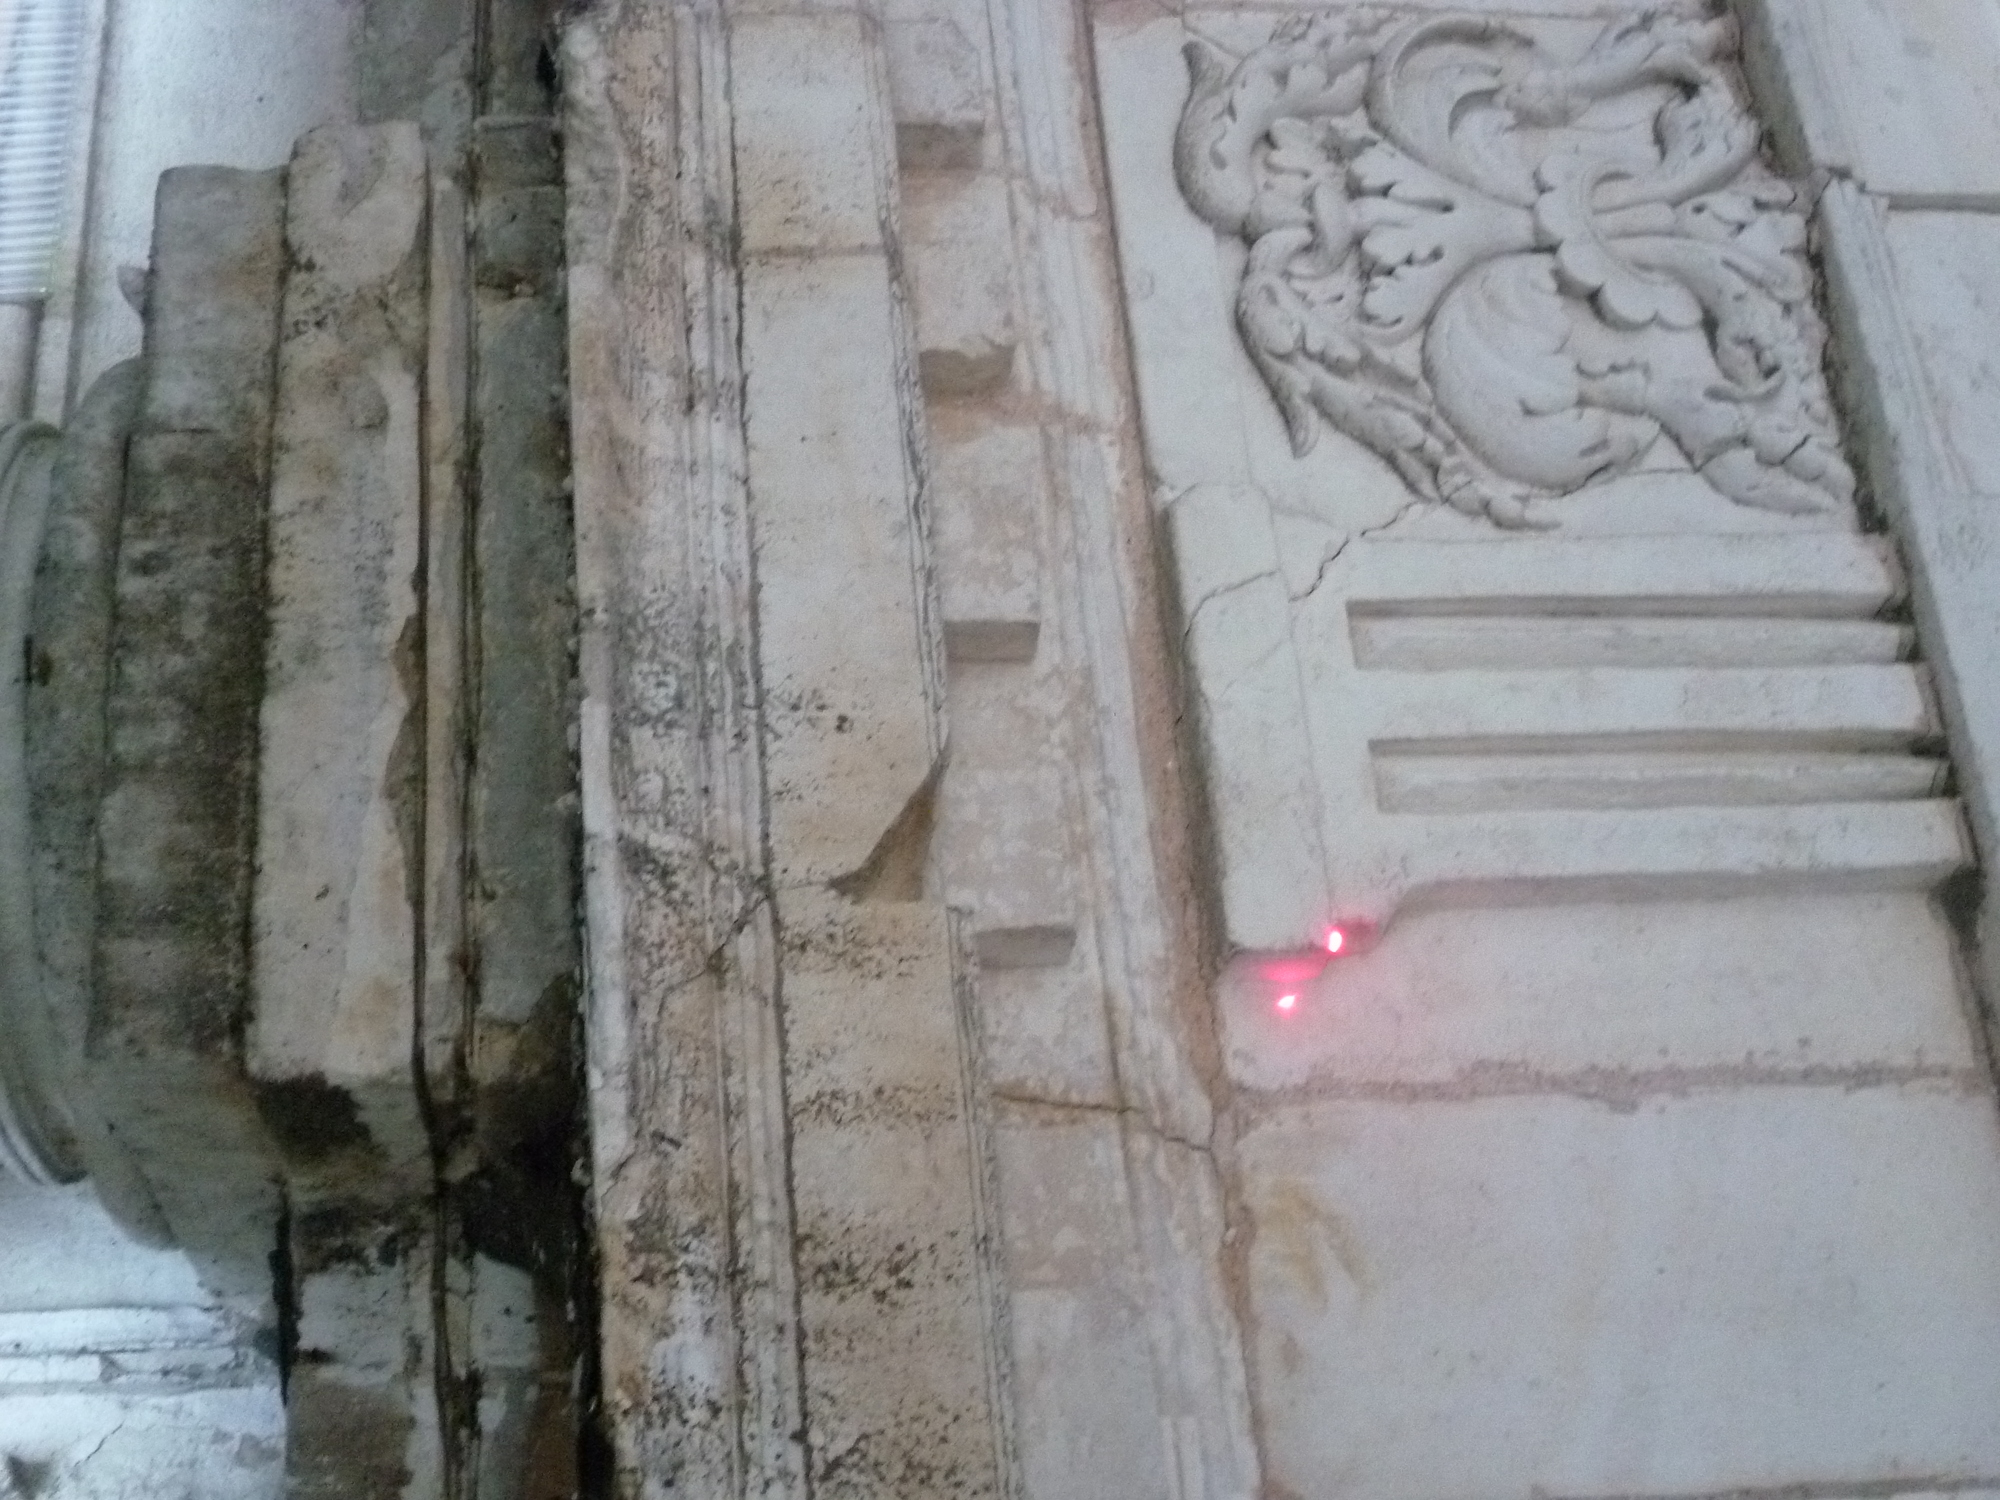
\includegraphics[bb=0 0 2880 2160,trim=0 0 400 300,width=500pt,keepaspectratio=true]{photo538.JPG}
%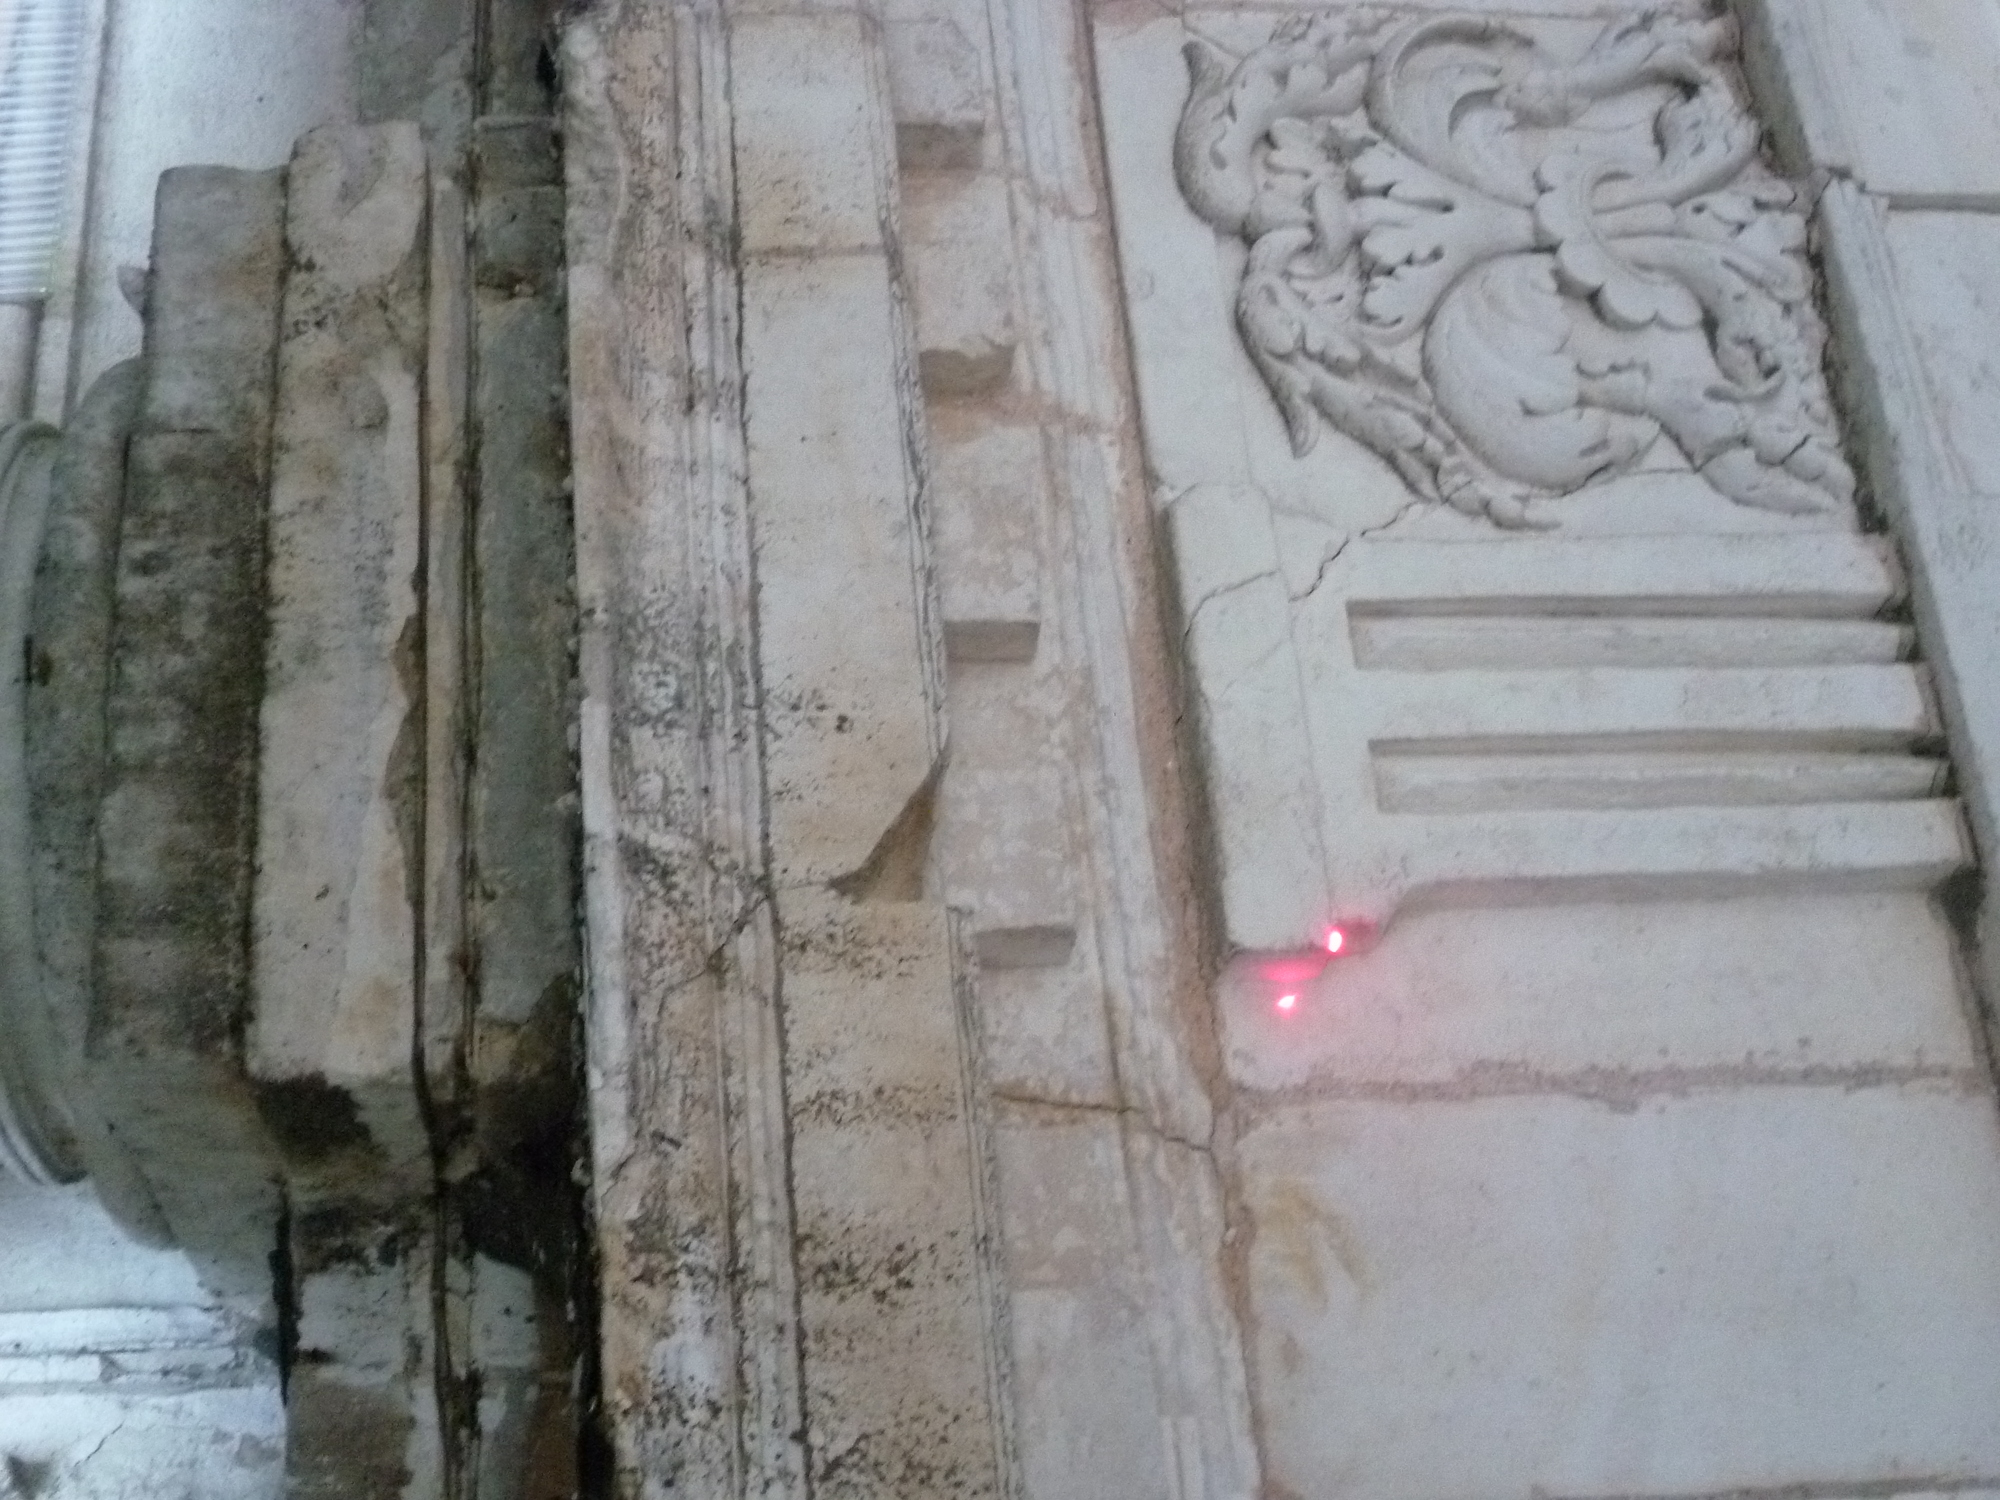
\includegraphics[trim=0 0 100 100,width=300pt,keepaspectratio=true]{photo538.JPG}
%
\includegraphics[bb=0 0 400 300,width=400pt,keepaspectratio=true]{test.jpg}
%
\includegraphics[bb=0 0 400 300,viewport=0 0 400 300,width=400pt,keepaspectratio=true]{test.jpg}
%
\includegraphics[bb=0 0 400 300,trim=0 0 399 299,width=400pt,keepaspectratio=true]{test.jpg}
%\includegraphics[trim=0 0 3000 2000,width=300pt,keepaspectratio=true]{P1020538.JPG}
%\includegraphics[width=100pt]{p1020538.jpg}
%\caption{Point 1009}
%\label{mydessin1}
%\end{figure}

\begin{figure}[h]
    \centering
    \begin{subfigure}[b]{0.3\textwidth}
        
\includegraphics[bb=0 0 400 300,height=3cm]{test.jpg}
        \caption{bb=0 0 400 300}
        \label{essai_1}
    \end{subfigure}
    ~ %add desired spacing between images, e. g. ~, \quad, \qquad etc.
      %(or a blank line to force the subfigure onto a new line)
    \begin{subfigure}[b]{0.3\textwidth}
        
\includegraphics[bb=0 0 400 300,height=3cm]{test.jpg}
        \caption{bb=0 0 400 300}
        \label{essai_2}
    \end{subfigure}
    ~
    \begin{subfigure}[b]{0.3\textwidth}
        
\includegraphics[bb=0 0 400 300,height=3cm]{test.jpg}
        \caption{bb=0 0 400 300}
        \label{essai_3}
    \end{subfigure}
    \\
    \begin{subfigure}[b]{0.3\textwidth}
        
\includegraphics[bb=0 0 400 300,height=3cm]{test.jpg}
        \caption{bb=0 0 400 300}
        \label{essai_4}
    \end{subfigure}
    ~ %add desired spacing between images, e. g. ~, \quad, \qquad etc.
      %(or a blank line to force the subfigure onto a new line)
    \begin{subfigure}[b]{0.3\textwidth}
        
\includegraphics[bb=0 0 400 300,height=3cm]{test.jpg}
        \caption{bb=0 0 400 300}
        \label{essai_5}
    \end{subfigure}
    ~
    \begin{subfigure}[b]{0.3\textwidth}
        
\includegraphics[bb=0 0 400 300,height=3cm]{test.jpg}
        \caption{bb=0 0 400 300}
        \label{essai_6}
    \end{subfigure}
    \caption{Les options pour l'insertion d'une image}%\label{fig-double}
    \label{fig:Les options}

\end{figure}




% debut d'une seconde figure
\begin{figure}[!h]
\centering
%
\includegraphics[width=\textwidth]{mydessin.pdf}

\includegraphics[width=200pt]{mydessin.pdf}
\caption{Ceci est aussi mydessin.pdf}
\label{mydessin2}
\end{figure}

% debut d'une troisieme figure
\begin{figure}[!h]
\centering
%
\includegraphics[width=\textwidth]{mydessin.pdf}

\includegraphics[width=300pt]{mydessin.pdf}
\caption{Ceci est encore mydessin.pdf}
\label{mydessin3}
\end{figure}

% debut d'une quatrieme figure
\begin{figure}[!h]
\centering
%
\includegraphics[width=\textwidth]{mydessin.pdf}

\includegraphics[width=400pt]{mydessin.pdf}
\caption{Ceci est encore et toujours mydessin.pdf}
\label{mydessin4}
\end{figure}

% reference a une figure
Sur la figure~\ref{mydessin1}, page~\pageref{mydessin1}, nous avons mis une largeur de 100 pt.

Sur la figure~\ref{mydessin2}, page~\pageref{mydessin2}, nous avons mis une largeur de 200 pt.

Sur la figure~\ref{mydessin3}, page~\pageref{mydessin3}, nous avons mis une largeur de 300 pt.

Sur la figure~\ref{mydessin4}, page~\pageref{mydessin4}, nous avons mis une largeur de 400 pt.

% liste des figures
\listoffigures

\end{document}
